% :contentReference[oaicite:0]{index=0}
\documentclass[12pt]{article}
\usepackage[margin=1in]{geometry}
\usepackage{amsmath,amssymb,mathtools}
\usepackage{enumitem}
\usepackage{bm}
\usepackage{hyperref}
\usepackage{fancyhdr}
\usepackage{draftwatermark}
\usepackage{xcolor}
\usepackage{pgfplots}
\usepackage{titlesec}
\pgfplotsset{compat=newest}

%------------- TITLE AND METADATA -------------

\newcommand{\CourseCode}{HE2001 }
\newcommand{\CourseName}{Microeconomics II}
\newcommand{\DocType}{Tutorial 5}

\title{
\CourseCode \CourseName \\[0.3em]
\large \DocType
}
\author{
  Academic Year 2025/2026, Semester 2 \\[0.25em]
  \textit{Quantitative Research Society @NTU}
}
\date{\today}

%------------- HEADER & FOOTER (for page 2 onward) -------------
\fancypagestyle{main}{
  \fancyhf{}
  \fancyhead[L]{\CourseCode \CourseName \ --\ \DocType}
  \fancyhead[R]{\href{https://qrsntu.org}{QRS@NTU}}
  \fancyfoot[C]{\thepage}
  \renewcommand{\headrulewidth}{0.4pt}
  \renewcommand{\footrulewidth}{0pt}
}

%------------- SIMPLE FOOTER (page 1 only) -------------
\fancypagestyle{plainfirst}{
  \fancyhf{}
  \renewcommand{\headrulewidth}{0pt}
  \renewcommand{\footrulewidth}{0pt}
  \fancyfoot[C]{\scriptsize\textcolor{gray}{\textit{For academic reference only. This document is provided for educational purposes and does not constitute an official question paper, answer key, or any formally authorised academic material. Its content is not guaranteed to be complete or accurate.}}}
}

%------------- WATERMARK -------------
\SetWatermarkText{Unofficial — QRS@NTU — qrsntu.org}
\SetWatermarkScale{1}
\SetWatermarkLightness{0.99}
%------------------------------------

%------------- SHORTCUTS -------------
\newcommand{\R}{\mathbb{R}}
\newcommand{\Rp}{\mathbb{R}_+}
\newcommand{\E}{\mathbb{E}}
\newcommand{\Var}{\mathrm{Var}}
\newcommand{\dotp}{\cdot}
%------------------------------------

%------------- Table of Contents -------------
\setcounter{tocdepth}{3}     % Ensures \subsubsection level shows in TOC
%------------------------------------


\begin{document}

\maketitle
\thispagestyle{plainfirst}
\pagestyle{main}
\bigskip

%====================================================
% OVERVIEW
%====================================================
\begin{center}
  \rule{0.8\textwidth}{0.4pt}\\[4pt]
  \textbf{Overview}\\[2pt]
  \rule{0.8\textwidth}{0.4pt}
\end{center}

\noindent
This tutorial covers:
\begin{itemize}[leftmargin=*]
  \item taxes and no-arbitrage rates of return;
  \item contingent consumption, spanning, and portfolio feasibility (with/without short sales);
  \item state prices and replication pricing;
  \item insurance as a contingent-claims market restriction and budget geometry;
  \item expected-utility (EU) maximisation and demand for state-contingent consumption.
\end{itemize}

\bigskip

%====================================================
% Table Of Contents
%====================================================
\newpage
\tableofcontents

%====================================================
% PART 1
%====================================================
\newpage
\section{Taxes}

\subsection{After-tax vs pre-tax returns}
There are two assets A and B. Asset A is not taxed whereas asset B is taxed on its returns.
Let \(r\) be the interest rate and \(\tau\) be the tax rate. Neither asset pays out any money in period
0.

Calculate rates of return \(\frac{p^A_1}{p^A_0}-1\) and \(\frac{p^B_1}{p^B_0}-1\) (where \(p^k_t\)
is the price of asset \(k\) in period \(t\)).

\subsection*{Solution}
\subsubsection*{Method 1: No-arbitrage using after-tax returns}
\paragraph{Asset \(A\).}
Asset \(A\) has no taxes. Its (gross) return is \(\frac{p^A_1}{p^A_0}\), so its net rate of return is
\[
R_A=\frac{p^A_1}{p^A_0}-1.
\]
Since \(r\) is the (relevant) interest rate, no-arbitrage requires \(R_A=r\), hence
\[
\frac{p^A_1}{p^A_0}-1=r.
\]

\paragraph{Asset \(B\).}
Asset \(B\) is taxed on its \emph{returns}. Interpreting this as a proportional tax \(\tau\) on the net return,
the \emph{after-tax} return is
\[
(1-\tau)\left(\frac{p^B_1}{p^B_0}-1\right).
\]
No-arbitrage requires the after-tax return equals the interest rate \(r\):
\[
(1-\tau)\left(\frac{p^B_1}{p^B_0}-1\right)=r
\quad\Rightarrow\quad
\frac{p^B_1}{p^B_0}-1=\frac{r}{1-\tau}.
\]

\[
\boxed{\;\frac{p^A_1}{p^A_0}-1=r,\qquad \frac{p^B_1}{p^B_0}-1=\frac{r}{1-\tau}\;}
\]

\subsubsection*{Method 2: Replication by borrowing/lending and tax wedge}
If asset \(A\) is untaxed, it can be used as the benchmark risk-free asset (or equivalently saving/borrowing at rate \(r\)).
Thus \(A\) must satisfy \(\frac{p^A_1}{p^A_0}=1+r\), i.e. \(\frac{p^A_1}{p^A_0}-1=r\).

For \(B\), an investor who buys \(B\) receives a pre-tax net return \(\frac{p^B_1}{p^B_0}-1\) but keeps only a fraction \(1-\tau\).
Therefore its after-tax return is \((1-\tau)\left(\frac{p^B_1}{p^B_0}-1\right)\).
To avoid arbitrage relative to the risk-free rate \(r\), we must have
\[
(1-\tau)\left(\frac{p^B_1}{p^B_0}-1\right)=r,
\]
yielding the same result.
\[
\boxed{\;\frac{p^A_1}{p^A_0}-1=r,\qquad \frac{p^B_1}{p^B_0}-1=\frac{r}{1-\tau}\;}
\]

\subsection{Dividend on untaxed asset}
Now, suppose asset A pays out \(y_0\) in period 0. This dividend is un-taxed. Calculate
\(\frac{p^A_1}{p^A_0}-1\).

\subsection*{Solution}
\subsubsection*{Method 1: Return definition with a period-0 dividend}
Buying \(A\) at price \(p^A_0\) and receiving an untaxed dividend \(y_0\) in period 0 means the \emph{net} outlay at \(t=0\) is
\[
p^A_0-y_0.
\]
There is no other payoff until resale at \(t=1\) for \(p^A_1\). Thus the (net) rate of return is
\[
r=\frac{p^A_1-(p^A_0-y_0)}{p^A_0-y_0}.
\]
Rearrange:
\[
p^A_1=(1+r)(p^A_0-y_0).
\]
Hence
\[
\frac{p^A_1}{p^A_0}-1
=\frac{(1+r)(p^A_0-y_0)}{p^A_0}-1
=(1+r)\left(1-\frac{y_0}{p^A_0}\right)-1
=r-\frac{(1+r)y_0}{p^A_0}.
\]

\[
\boxed{\;\frac{p^A_1}{p^A_0}-1=r-\frac{(1+r)y_0}{p^A_0}\;}
\]

\subsubsection*{Method 2: Present-value identity then convert to the requested return}
No-arbitrage implies the time-0 price equals the present value of time-1 resale plus the time-0 dividend (which is already in present value):
\[
p^A_0=y_0+\frac{p^A_1}{1+r}
\quad\Rightarrow\quad
p^A_1=(1+r)(p^A_0-y_0).
\]
Then
\[
\frac{p^A_1}{p^A_0}-1=\frac{(1+r)(p^A_0-y_0)}{p^A_0}-1
=r-\frac{(1+r)y_0}{p^A_0},
\]
as above.
\[
\boxed{\;\frac{p^A_1}{p^A_0}-1=r-\frac{(1+r)y_0}{p^A_0}\;}
\]

\subsection{Dividend on taxed asset}
Now, suppose asset B pays out \(y_0\) in period 0. This dividend is un-taxed. Calculate
\(\frac{p^B_1}{p^B_0}-1\).

\subsection*{Solution}
\subsubsection*{Method 1: After-tax return equals \(r\) with untaxed dividend}
Dividend \(y_0\) at \(t=0\) is untaxed, so the net outlay is \(p^B_0-y_0\).
Asset \(B\) is taxed on its returns, so the after-tax net return on the net investment is
\[
(1-\tau)\left(\frac{p^B_1-(p^B_0-y_0)}{p^B_0-y_0}\right).
\]
No-arbitrage requires this after-tax return equals \(r\):
\[
(1-\tau)\left(\frac{p^B_1-(p^B_0-y_0)}{p^B_0-y_0}\right)=r.
\]
Solve:
\[
\frac{p^B_1-(p^B_0-y_0)}{p^B_0-y_0}=\frac{r}{1-\tau}
\quad\Rightarrow\quad
p^B_1=\left(1+\frac{r}{1-\tau}\right)(p^B_0-y_0).
\]
Therefore
\[
\frac{p^B_1}{p^B_0}-1
=\left(1+\frac{r}{1-\tau}\right)\left(1-\frac{y_0}{p^B_0}\right)-1.
\]

\[
\boxed{\;\frac{p^B_1}{p^B_0}-1=\left(1+\frac{r}{1-\tau}\right)\left(1-\frac{y_0}{p^B_0}\right)-1\;}
\]

\subsubsection*{Method 2: Rewrite using pre-tax return wedge}
Let the pre-tax rate of return on the net investment be
\[
R_B^{\text{pre}}=\frac{p^B_1-(p^B_0-y_0)}{p^B_0-y_0}.
\]
Taxation implies after-tax return \(R_B^{\text{aft}}=(1-\tau)R_B^{\text{pre}}\). No-arbitrage gives \(R_B^{\text{aft}}=r\), hence
\[
R_B^{\text{pre}}=\frac{r}{1-\tau}.
\]
Thus \(p^B_1=(1+R_B^{\text{pre}})(p^B_0-y_0)=\left(1+\frac{r}{1-\tau}\right)(p^B_0-y_0)\), and
\[
\frac{p^B_1}{p^B_0}-1=\left(1+\frac{r}{1-\tau}\right)\left(1-\frac{y_0}{p^B_0}\right)-1.
\]
\[
\boxed{\;\frac{p^B_1}{p^B_0}-1=\left(1+\frac{r}{1-\tau}\right)\left(1-\frac{y_0}{p^B_0}\right)-1\;}
\]

%====================================================
% PART 2
%====================================================
\newpage
\section{Contingent Consumption and Assets}

Suppose there are two equally likely states: \(S=2\) and \(\pi=\left(\frac12,\frac12\right)\).

\subsection{Expected values in two states}
What is the expected value of \(x=(5,3)\) and \(x^{1}=(2,8)\)?

\subsection*{Solution}
\subsubsection*{Method 1: Direct computation}
\[
\E[x]=\frac12\cdot 5+\frac12\cdot 3=\frac{8}{2}=4,
\qquad
\E[x^{1}]=\frac12\cdot 2+\frac12\cdot 8=\frac{10}{2}=5.
\]
\[
\boxed{\;\E[x]=4,\qquad \E[x^{1}]=5\;}
\]

\subsubsection*{Method 2: Use the midpoint property under equal probabilities}
With two equally likely states, the expectation is the midpoint of the two state values:
\[
\E[(a,b)]=\frac{a+b}{2}.
\]
So \(\E[(5,3)]=(5+3)/2=4\) and \(\E[(2,8)]=(2+8)/2=5\).
\[
\boxed{\;\E[x]=4,\qquad \E[x^{1}]=5\;}
\]

\subsection{Affordability with state prices}
Suppose can buy contingent consumption directly at prices \(p=(1,4)\). Suppose the
consumer can spend 6. Can the consumer afford \((2,1)\)? What about \((1,2)\)?

\subsection*{Solution}
\subsubsection*{Method 1: Compute costs}
Cost of \((2,1)\):
\[
p\dotp (2,1)=1\cdot 2+4\cdot 1=6 \le 6 \quad\Rightarrow\quad \text{affordable}.
\]
Cost of \((1,2)\):
\[
p\dotp (1,2)=1\cdot 1+4\cdot 2=9>6 \quad\Rightarrow\quad \text{not affordable}.
\]
\[
\boxed{\;(2,1)\text{ is affordable; }(1,2)\text{ is not affordable.}\;}
\]

\subsubsection*{Method 2: Budget-line inequality}
Affordable set is \(\{(x_1,x_2)\in\Rp^2: x_1+4x_2\le 6\}\).
Check:
\[
2+4\cdot 1=6\le 6 \Rightarrow (2,1)\in B,
\qquad
1+4\cdot 2=9>6 \Rightarrow (1,2)\notin B.
\]
\[
\boxed{\;(2,1)\text{ is affordable; }(1,2)\text{ is not affordable.}\;}
\]

\subsection{Portfolio feasibility without short sales}
Now, suppose you cannot buy contingent consumption directly. Suppose there are two
assets: a risk free asset \(a^f=(1,1)\) and a risky asset \(a^r=(4,1)\). The risk free asset costs
1 and the risky asset costs 2. Suppose you cannot short and suppose the consumer has
3 to spend. Can the consumer afford the contingent consumption bundle \((5,2)\)? What
about \((4,4)\)? What about \((2,3)\)?

\subsection*{Solution}
Let holdings be \(\theta=(\theta_f,\theta_r)\) with \(\theta_f\ge 0,\theta_r\ge 0\) (no shorting).
Cost constraint:
\[
\theta_f+2\theta_r\le 3.
\]
Delivered consumption:
\[
\theta_f a^f+\theta_r a^r=(\theta_f+4\theta_r,\ \theta_f+\theta_r).
\]

\subsubsection*{Method 1: Solve replication system and check constraints}
\paragraph{Target \((5,2)\).}
Solve
\[
\theta_f+4\theta_r=5,\qquad \theta_f+\theta_r=2.
\]
Subtract: \(3\theta_r=3\Rightarrow \theta_r=1\), hence \(\theta_f=1\).
Cost \(=1+2=3\le 3\) and nonnegativity holds, so affordable.

\paragraph{Target \((4,4)\).}
Solve
\[
\theta_f+4\theta_r=4,\qquad \theta_f+\theta_r=4.
\]
Subtract: \(3\theta_r=0\Rightarrow \theta_r=0\), hence \(\theta_f=4\).
Cost \(=4>3\), not affordable.

\paragraph{Target \((2,3)\).}
Solve
\[
\theta_f+4\theta_r=2,\qquad \theta_f+\theta_r=3.
\]
Subtract: \(3\theta_r=-1\Rightarrow \theta_r=-\frac{1}{3}\), which violates \(\theta_r\ge 0\). Not affordable.

\[
\boxed{\;(5,2)\text{ affordable; }(4,4)\text{ not affordable; }(2,3)\text{ not affordable.}\;}
\]

\subsubsection*{Method 2: Feasible set geometry in payoff space}
Payoff set from \(\theta_f,\theta_r\ge 0\) with \(\theta_f+2\theta_r\le 3\) is the convex hull of the payoffs at the budget corners:
\[
(\theta_f,\theta_r)=(0,0)\Rightarrow (0,0),
\quad
(3,0)\Rightarrow (3,3),
\quad
(0,1.5)\Rightarrow (6,1.5).
\]
Thus feasible contingent consumption bundles are all convex combinations of \((0,0),(3,3),(6,1.5)\).

Check:
\begin{itemize}[leftmargin=*]
\item \((5,2)\) lies on the segment between \((3,3)\) and \((6,1.5)\): indeed \((5,2)=(3,3)+\frac{2}{3}(3,-1.5)\), corresponding to \((\theta_f,\theta_r)=(1,1)\).
\item \((4,4)\) has second component 4, but the feasible set has \(x_2\le 3\) when \(\theta_f+2\theta_r\le 3\) and \(\theta\ge 0\) (since \(x_2=\theta_f+\theta_r\le \theta_f+2\theta_r\le 3\)). So impossible.
\item \((2,3)\) requires \(x_2=3\) but \(x_1=2\); with \(\theta_f,\theta_r\ge 0\), \(x_1=\theta_f+4\theta_r\ge \theta_f+\theta_r=x_2\), so \(x_1<x_2\) is impossible. Hence not affordable.
\end{itemize}
\[
\boxed{\;(5,2)\text{ affordable; }(4,4)\text{ not affordable; }(2,3)\text{ not affordable.}\;}
\]

\subsection{State prices from spanning with short sales}
Now, suppose that the assets can be held short. Find the state price vector \(p=(p_1,p_2)\).
That is, \(p\) is the price of contingent consumption so that, for any \(\theta=(\theta_f,\theta_r)\) the price
of \(\theta\) is the same as the price of the contingent consumption delivered by \(\theta\):
\[
\theta_f+2\theta_r=p\dotp\bigl(\theta_f a^f+\theta_r a^r\bigr),\ \ \text{for all }\theta_f,\theta_r.
\]
Hint: take \(\theta=(1,0)\) and \(\theta=(0,1)\) and solve for \((p_1,p_2)\). This is two equations and two
unknowns.

\subsection*{Solution}
\subsubsection*{Method 1: Use the hint \(\theta=(1,0)\) and \(\theta=(0,1)\)}
For \(\theta=(1,0)\), LHS price is \(1\). Delivered bundle is \(a^f=(1,1)\), so
\[
1=p\dotp(1,1)=p_1+p_2. \tag{A}
\]
For \(\theta=(0,1)\), LHS price is \(2\). Delivered bundle is \(a^r=(4,1)\), so
\[
2=p\dotp(4,1)=4p_1+p_2. \tag{B}
\]
Subtract (A) from (B): \(3p_1=1\Rightarrow p_1=\frac{1}{3}\).
Then \(p_2=1-p_1=\frac{2}{3}\).

\[
\boxed{\;p=\left(\frac13,\frac23\right)\;}
\]

\subsubsection*{Method 2: Coefficient matching for all \(\theta_f,\theta_r\)}
We require for all \((\theta_f,\theta_r)\in\R^2\):
\[
\theta_f+2\theta_r
=p\dotp\bigl(\theta_f(1,1)+\theta_r(4,1)\bigr)
=\theta_f(p_1+p_2)+\theta_r(4p_1+p_2).
\]
Matching coefficients of \(\theta_f\) and \(\theta_r\) gives the same system:
\[
p_1+p_2=1,\qquad 4p_1+p_2=2,
\]
so \(p_1=\frac13\), \(p_2=\frac23\).
\[
\boxed{\;p=\left(\frac13,\frac23\right)\;}
\]

\subsection{Replicating a target bundle and pricing}
Suppose you want to buy contingent consumption \((6,3)\). How much of each asset do
you need to purchase? How much does this cost? How much does \((6,3)\) cost according
to the state prices \(p=(p_1,p_2)\) you found in the previous question?

\subsection*{Solution}
\subsubsection*{Method 1: Replication by solving for \(\theta_f,\theta_r\)}
We need
\[
\theta_f+4\theta_r=6,\qquad \theta_f+\theta_r=3.
\]
Subtract: \(3\theta_r=3\Rightarrow \theta_r=1\). Then \(\theta_f=2\).

Portfolio cost:
\[
\theta_f+2\theta_r=2+2=4.
\]
State-price cost using \(p=(1/3,2/3)\):
\[
p\dotp(6,3)=\frac13\cdot 6+\frac23\cdot 3=2+2=4.
\]
\[
\boxed{\;\theta_f=2,\ \theta_r=1;\ \text{cost}=4;\ \text{state-price cost}=4.\;}
\]

\subsubsection*{Method 2: Use spanning/pricing identity directly}
Since state prices satisfy
\[
\theta_f+2\theta_r=p\dotp(\theta_f a^f+\theta_r a^r),
\]
any replicable bundle is priced by \(p\). If \((6,3)\) is replicated by \((\theta_f,\theta_r)\), then its cost equals \(p\dotp(6,3)\).
Compute
\[
p\dotp(6,3)=\frac13\cdot 6+\frac23\cdot 3=4.
\]
To find holdings, solve the payoff system:
\[
\theta_f+\theta_r=3,\ \theta_f+4\theta_r=6\Rightarrow \theta_r=1,\ \theta_f=2,
\]
and the portfolio cost is \(2+2=4\), matching \(p\dotp(6,3)\).
\[
\boxed{\;\theta_f=2,\ \theta_r=1;\ \text{cost}=4.\;}
\]

%====================================================
% PART 3
%====================================================
\newpage
\section{Contingent Consumption and Insurance}

Suppose there are two states where the first state has probability \(\frac13\): \(S=2\) and \(\pi=\left(\frac13,\frac23\right)\).

\subsection{Expected values with unequal probabilities}
What is the expected value of \(x=(6,3)\) and \(x^{1}=(9,12)\).

\subsection*{Solution}
\subsubsection*{Method 1: Direct computation}
\[
\E[x]=\frac13\cdot 6+\frac23\cdot 3=2+2=4,
\qquad
\E[x^{1}]=\frac13\cdot 9+\frac23\cdot 12=3+8=11.
\]
\[
\boxed{\;\E[x]=4,\qquad \E[x^{1}]=11\;}
\]

\subsubsection*{Method 2: Weighted-average form}
For \(\pi=(1/3,2/3)\),
\[
\E[(a,b)]=\frac{a+2b}{3}.
\]
So \(\E[(6,3)]=(6+2\cdot 3)/3=12/3=4\) and \(\E[(9,12)]=(9+2\cdot 12)/3=33/3=11\).
\[
\boxed{\;\E[x]=4,\qquad \E[x^{1}]=11\;}
\]

\subsection{Endowment vs expected value under concave utility}
Suppose the consumer has utility function \(U(x_1,x_2)=\frac13u(x_1)+\frac23u(x_2)\) where \(u(x)=\sqrt{x}\) and suppose the consumer is endowed with \(\omega=(0,9)\). Does the consumer prefer his endowment or its expected value: \(x=(6,6)\)?

\subsection*{Solution}
\subsubsection*{Method 1: Compute expected utility exactly}
Compute EU of endowment:
\[
U(\omega)=\frac13\sqrt{0}+\frac23\sqrt{9}=0+\frac23\cdot 3=2.
\]
Compute EU of \(x=(6,6)\):
\[
U(x)=\frac13\sqrt{6}+\frac23\sqrt{6}=\sqrt{6}.
\]
Since \(\sqrt{6}>2\) (square both sides: \(6>4\)), we have \(U(x)>U(\omega)\).

\[
\boxed{\;\text{The consumer prefers }(6,6)\text{ to }\omega=(0,9).\;}
\]

\subsubsection*{Method 2: Jensen's inequality intuition plus verification}
Because \(u(x)=\sqrt{x}\) is strictly concave, equalising consumption across states increases expected utility relative to a spread, holding mean fixed. Here \((6,6)\) is fully equalised and the endowment is highly unequal. A direct check confirms:
\[
U(6,6)=\sqrt{6}>2=U(0,9).
\]
\[
\boxed{\;\text{Prefer the expected value bundle }(6,6).\;}
\]

\subsection{Affordable safe bundle using insurance}
Suppose the consumer can buy insurance. Specifically, can buy consumption in state 1
at the cost of one unit of consumption in state 2. That is, insurance is an asset \((1,-1)\).
Find the safe bundle \((k,k)\) (for some value of \(k\)) that the consumer can afford. Does
the consumer prefer this bundle or the endowment?

\subsection*{Solution}
Starting from \(\omega=(0,9)\), buying \(\theta\) units of insurance \((1,-1)\) yields
\[
x(\theta)=(\omega_1+\theta,\ \omega_2-\theta)=(\theta,\ 9-\theta).
\]
A safe bundle satisfies \(\theta=9-\theta\Rightarrow \theta=\frac{9}{2}\), hence
\[
k=\theta=\frac{9}{2}.
\]
So the affordable safe bundle is \(\left(\frac{9}{2},\frac{9}{2}\right)\).

Now compare utilities:
\[
U\!\left(\frac{9}{2},\frac{9}{2}\right)=\frac13\sqrt{\frac{9}{2}}+\frac23\sqrt{\frac{9}{2}}=\sqrt{\frac{9}{2}}=\frac{3}{\sqrt{2}},
\]
\[
U(\omega)=2.
\]
Since \(\frac{3}{\sqrt{2}}>2\) (square both sides: \(9/2>4\iff 9>8\)), the safe bundle is preferred.

\[
\boxed{\;k=\frac{9}{2},\ \text{so the safe bundle is }\left(\frac{9}{2},\frac{9}{2}\right),\ \text{and it is preferred to }\omega.\;}
\]

\subsubsection*{Method 2: Feasible set midpoint and concavity}
The budget set generated by \((1,-1)\) from \(\omega\) is the line \(x_1+x_2=9\). The safe bundle is the midpoint of the segment where \(x_1=x_2\), hence \(k=9/2\). Since \(u\) is strictly concave, equalisation increases utility, so the safe bundle dominates \(\omega\); the exact inequality check above confirms.
\[
\boxed{\;k=\frac{9}{2}\ \text{and the safe bundle is preferred.}\;}
\]

\subsection{Budget line with insurance}
Draw a picture of all the contingent consumption bundles which are affordable (i.e.
draw the budget line).

\subsection*{Solution}
\subsubsection*{Method 1: Parametric form and intercepts}
Affordable bundles are \(x(\theta)=(\theta,9-\theta)\). Eliminating \(\theta\) gives
\[
x_1+x_2=9.
\]
If we restrict to nonnegative consumption, then \(x_1\in[0,9]\) and \(x_2=9-x_1\), with intercepts \((0,9)\) and \((9,0)\).
\[
\boxed{\;\text{Budget line: }x_2=9-x_1\ \text{(in }\Rp^2\text{, the segment from }(0,9)\text{ to }(9,0)).\;}
\]

\begin{figure}[htpb]
    \centering
    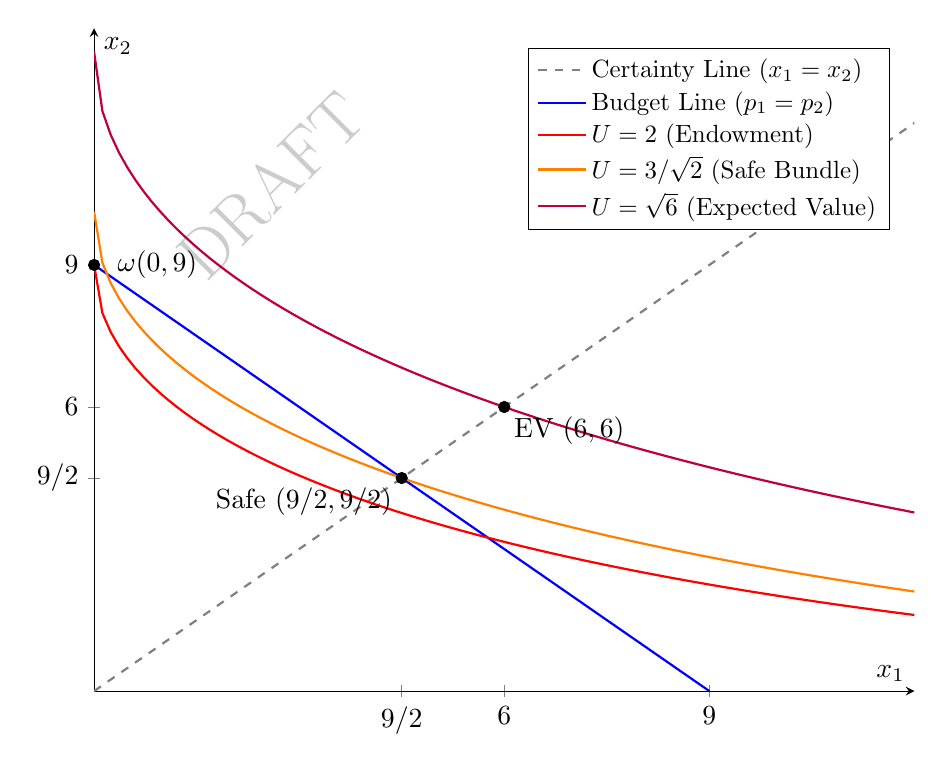
\begin{tikzpicture}
        \begin{axis}[
            axis lines = center,
            xlabel = {$x_1$},
            ylabel = {$x_2$},
            xmin = 0, xmax = 12,
            ymin = 0, ymax = 14,
            xtick = {4.5, 6, 9},
            xticklabels = {$9/2$, 6, 9},
            ytick = {4.5, 6, 9},
            yticklabels = {$9/2$, 6, 9},
            legend pos = north east,
            legend cell align = {left},
            legend style={nodes={scale=0.9, transform shape}},
            grid = none,
            width = 12cm,
            height = 10cm,
            % Ensure indifference curves are smooth
            samples = 100
        ]
        
        % 45-degree Certainty Line
        \addplot [domain=0:12, dashed, gray, thick] {x};
        \addlegendentry{Certainty Line ($x_1=x_2$)}
        
        % Budget Line (x_1 + x_2 = 9)
        \addplot [domain=0:9, thick, blue] {9 - x};
        \addlegendentry{Budget Line ($p_1=p_2$)}
        
        % Indifference Curve 1: Through Endowment U = 2
        % Derivation: (1/3)sqrt(x_1) + (2/3)sqrt(x_2) = 2 => x_2 = (3 - 0.5*sqrt(x_1))^2
        \addplot [domain=0:12, thick, red] {(3 - 0.5*sqrt(x))^2};
        \addlegendentry{$U=2$ (Endowment)}
        
        % Indifference Curve 2: Through Safe Bundle U = 3/\sqrt{2} \approx 2.12
        % Derivation: x_2 = (4.5/sqrt(2) - 0.5*sqrt(x_1))^2
        \addplot [domain=0:12, thick, orange] {(4.5/sqrt(2) - 0.5*sqrt(x))^2};
        \addlegendentry{$U=3/\sqrt{2}$ (Safe Bundle)}
        
        % Indifference Curve 3: Through Expected Value (6,6) U = \sqrt{6} \approx 2.45
        % Derivation: x_2 = (1.5*sqrt(6) - 0.5*sqrt(x_1))^2
        \addplot [domain=0:12, thick, purple] {(1.5*sqrt(6) - 0.5*sqrt(x))^2};
        \addlegendentry{$U=\sqrt{6}$ (Expected Value)}
        
        % Points
        % 1. Endowment
        \addplot[mark=*, black] coordinates {(0,9)};
        \node[right] at (axis cs:0.2, 9) {$\omega(0,9)$};
        
        % 2. Safe Bundle
        \addplot[mark=*, black] coordinates {(4.5,4.5)};
        \node[below left] at (axis cs:4.5, 4.5) {Safe $(9/2, 9/2)$};
        
        % 3. Expected Value
        \addplot[mark=*, black] coordinates {(6,6)};
        \node[below right] at (axis cs:6, 6) {EV $(6,6)$};
        
        \end{axis}
    \end{tikzpicture}
    \caption{Affordable contingent consumption bundles, the certainty line, and indifference curves illustrating the preference for insurance and expected value over the endowment.}
    \label{fig:contingent_consumption}
\end{figure}

\subsubsection*{Method 2: Vector-geometry description}
The endowment is \(\omega=(0,9)\) and the trade direction is \((1,-1)\), so the affine line of attainable bundles is
\[
\omega+\mathrm{span}\{(1,-1)\}=\{(0,9)+\theta(1,-1):\theta\in\R\},
\]
i.e. \(x_1+x_2=9\). Restricting to \(\Rp^2\) gives the segment between the axis intercepts.
\[
\boxed{\;x_1+x_2=9\ \text{(restricted to nonnegative quadrant).}\;}
\]

\subsection{Price vectors constant on the budget line}
Can you find a price vector \(p=(p_1,p_2)\) so that the price of a contingent consumption
\(x\) is the same for every affordable contingent consumption bundle:
\[
p\dotp \omega = p\dotp(\omega_1+\theta,\omega_2-\theta),\ \ \text{for all }\theta?
\]
Note that there is more than one price vector \(p\) which satisfies this equality.

\subsection*{Solution}
We need \(p\dotp(\omega_1+\theta,\omega_2-\theta)\) to be independent of \(\theta\).

\subsubsection*{Method 1: Coefficient of \(\theta\) must be zero}
Compute:
\[
p\dotp(\omega_1+\theta,\omega_2-\theta)=p_1(\omega_1+\theta)+p_2(\omega_2-\theta)
=p_1\omega_1+p_2\omega_2+\theta(p_1-p_2).
\]
For this to equal \(p\dotp\omega=p_1\omega_1+p_2\omega_2\) for all \(\theta\), we require
\[
p_1-p_2=0\quad\Rightarrow\quad p_1=p_2.
\]
Thus any vector of the form \(p=(c,c)\) (with \(c\neq 0\), typically \(c>0\)) works.

\[
\boxed{\;\text{All solutions are }p=(c,c)\ \text{for any }c\neq 0\text{ (e.g. }p=(1,1)).\;}
\]

\subsubsection*{Method 2: Normal vector to the budget line}
The affordable set lies on the line \(x_1+x_2=9\), whose direction vector is \((1,-1)\).
A price vector that assigns the same value to all points on the line must be orthogonal to the direction, i.e.
\[
p\dotp(1,-1)=0\Rightarrow p_1-p_2=0\Rightarrow p_1=p_2.
\]
So \(p=(c,c)\) for any \(c\neq 0\).
\[
\boxed{\;p_1=p_2\ \text{(e.g. }p=(1,1)\text{).}\;}
\]

%====================================================
% PART 4
%====================================================
\newpage
\section{EU maximization}

Suppose there are two states (\(S=2\)) and that \(\pi=\left(\frac13,\frac23\right)\). Suppose utility takes the form
\[
U(x_1,x_2)=\frac13u(x_1)+\frac23u(x_2)
\]
where \(u(x)=\sqrt{x}\). We note that \(u'(x)=x^{-1/2}\).

\subsection{Marginal rate of substitution}
Find \(MRS_{1,2}\)?

\subsection*{Solution}
\subsubsection*{Method 1: Ratio of marginal utilities}
\[
\frac{\partial U}{\partial x_1}=\frac13 u'(x_1)=\frac13 x_1^{-1/2},\qquad
\frac{\partial U}{\partial x_2}=\frac23 u'(x_2)=\frac23 x_2^{-1/2}.
\]
Thus
\[
MRS_{1,2}=\frac{\partial U/\partial x_1}{\partial U/\partial x_2}
=\frac{\frac13 x_1^{-1/2}}{\frac23 x_2^{-1/2}}
=\frac12\cdot \frac{x_2^{-1/2}}{x_1^{-1/2}}
=\frac12\sqrt{\frac{x_2}{x_1}}.
\]
\[
\boxed{\;MRS_{1,2}=\frac12\sqrt{\frac{x_2}{x_1}}\;}
\]


\subsubsection*{Method 2: General formula with probabilities}
For EU, \(MRS_{1,2}=\frac{\pi_1 u'(x_1)}{\pi_2 u'(x_2)}\).
Here \(\pi_1/\pi_2=(1/3)/(2/3)=1/2\), so
\[
MRS_{1,2}=\frac12\cdot\frac{u'(x_1)}{u'(x_2)}
=\frac12\cdot\frac{x_1^{-1/2}}{x_2^{-1/2}}
=\frac12\sqrt{\frac{x_2}{x_1}}.
\]
\[
\boxed{\;MRS_{1,2}=\frac12\sqrt{\frac{x_2}{x_1}}\;}
\]

\newpage
\subsection{Demand with state prices}
Find the demand function for the consumer. That is, suppose you can buy contingent
consumption with price vector \(p=(p_1,p_2)\) and expenditure level \(m\). Find how much
contingent consumption is demanded for each price vector \(p\) and each \(m\).

\subsection*{Solution}
We maximise \(U(x_1,x_2)\) subject to \(p_1x_1+p_2x_2=m\), with \(x_1,x_2>0\).

\subsubsection*{Method 1: Lagrangian}
Lagrangian:
\[
\mathcal{L}=\frac13\sqrt{x_1}+\frac23\sqrt{x_2}+\lambda(m-p_1x_1-p_2x_2).
\]
FOCs:
\[
\frac{1}{3}\cdot\frac{1}{2\sqrt{x_1}}-\lambda p_1=0,\qquad
\frac{2}{3}\cdot\frac{1}{2\sqrt{x_2}}-\lambda p_2=0.
\]
Equivalently,
\[
\frac{1}{6\sqrt{x_1}}=\lambda p_1,\qquad \frac{1}{3\sqrt{x_2}}=\lambda p_2.
\]
Divide the first by the second:
\[
\frac{1}{6\sqrt{x_1}}\Big/\frac{1}{3\sqrt{x_2}}=\frac{\sqrt{x_2}}{2\sqrt{x_1}}=\frac{p_1}{p_2}
\quad\Rightarrow\quad
\sqrt{\frac{x_2}{x_1}}=\frac{2p_1}{p_2}
\quad\Rightarrow\quad
x_2=x_1\cdot \frac{4p_1^2}{p_2^2}.
\]
Use the budget:
\[
p_1x_1+p_2x_2=p_1x_1+p_2x_1\cdot\frac{4p_1^2}{p_2^2}
=x_1\left(p_1+\frac{4p_1^2}{p_2}\right)=m.
\]
Hence
\[
x_1(p,m)=\frac{m}{p_1+\frac{4p_1^2}{p_2}}
=\frac{m p_2}{p_1p_2+4p_1^2}
=\frac{m p_2}{p_1(p_2+4p_1)}.
\]
Then
\[
x_2(p,m)=\frac{4p_1^2}{p_2^2}\,x_1
=\frac{4p_1^2}{p_2^2}\cdot \frac{m p_2}{p_1(p_2+4p_1)}
=\frac{4p_1 m}{p_2(p_2+4p_1)}.
\]

\[
\boxed{\;x_1(p,m)=\frac{m p_2}{p_1(p_2+4p_1)},\qquad x_2(p,m)=\frac{4p_1 m}{p_2(p_2+4p_1)}\;}
\]

\subsubsection*{Method 2: Use MRS \(=\) price ratio}
Optimality requires
\[
MRS_{1,2}=\frac{p_1}{p_2}.
\]
From Question 4.1,
\[
\frac12\sqrt{\frac{x_2}{x_1}}=\frac{p_1}{p_2}
\quad\Rightarrow\quad
x_2=x_1\cdot\frac{4p_1^2}{p_2^2}.
\]
Substitute into the budget to solve \(x_1\), then obtain \(x_2\), yielding the same demand functions as Method 1.
\[
\boxed{\;x_1(p,m)=\frac{m p_2}{p_1(p_2+4p_1)},\qquad x_2(p,m)=\frac{4p_1 m}{p_2(p_2+4p_1)}\;}
\]

\subsection{Demand with given endowment and prices}
Suppose the consumer has endowment \(\omega=(0,9)\) and faces prices \(p=(2,1)\). What
contingent consumption bundle will the consumer buy?

\subsection*{Solution}
Expenditure equals the value of endowment:
\[
m=p\dotp\omega=2\cdot 0+1\cdot 9=9.
\]
Use the demand from Question 4.2 with \(p_1=2\), \(p_2=1\), \(m=9\):
\[
x_1=\frac{m p_2}{p_1(p_2+4p_1)}=\frac{9\cdot 1}{2(1+8)}=\frac{9}{18}=\frac12,
\]
\[
x_2=\frac{4p_1 m}{p_2(p_2+4p_1)}=\frac{4\cdot 2\cdot 9}{1(1+8)}=\frac{72}{9}=8.
\]
\[
\boxed{\;x=\left(\frac12,8\right)\;}
\]

\subsubsection*{Method 2: Use MRS condition then the budget}
At optimum,
\[
\frac12\sqrt{\frac{x_2}{x_1}}=\frac{p_1}{p_2}=\frac{2}{1}=2
\quad\Rightarrow\quad
\sqrt{\frac{x_2}{x_1}}=4
\quad\Rightarrow\quad
x_2=16x_1.
\]
Budget is \(2x_1+1\cdot x_2=m=9\), so \(2x_1+16x_1=18x_1=9\Rightarrow x_1=1/2\), hence \(x_2=8\).
\[
\boxed{\;x=\left(\frac12,8\right)\;}
\]

\subsection{Insurance-only trading}
Continue to assume that the consumer is endowed with \((0,9)\) but now the consumer
cannot purchase contingent consumption directly. Instead he can only buy insurance.
Each unit of insurance costs two units of consumption from state 2 and delivers 1 unit
of consumption in state 1. Draw the budget line of all consumption bundles which the
consumer can afford. How much contingent consumption will the consumer demand?
Hint: use the answer from the previous question.

\bigskip
\bigskip

\subsection*{Solution}
One unit of insurance transforms consumption by \((+1,-2)\). Starting from \(\omega=(0,9)\), buying \(\theta\) units yields
\[
x(\theta)=(\theta,\ 9-2\theta).
\]

\begin{figure}[htpb]
    \centering
    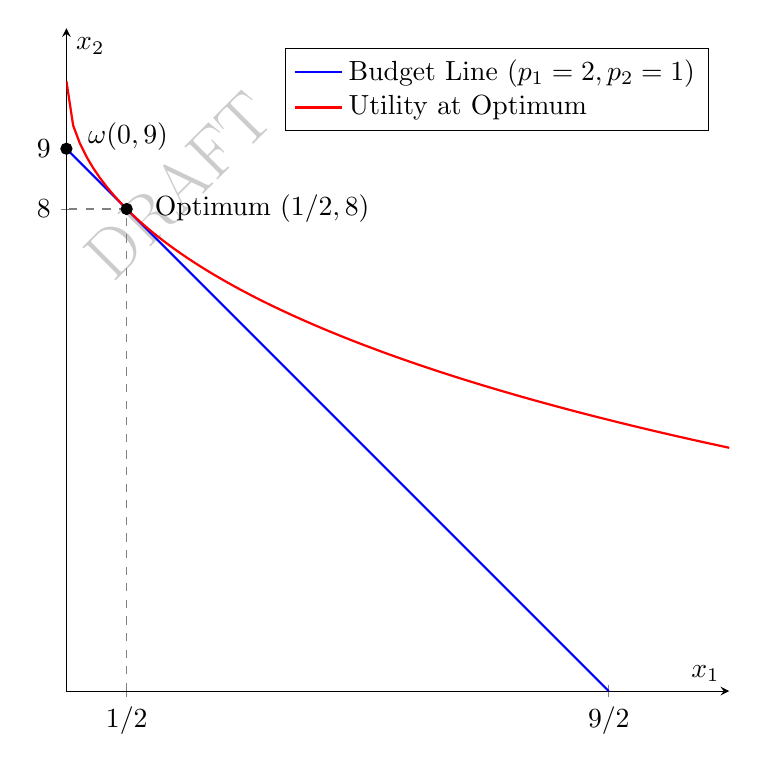
\begin{tikzpicture}
        \begin{axis}[
            axis lines = center,
            xlabel = {$x_1$},
            ylabel = {$x_2$},
            xmin = 0, xmax = 5.5,
            ymin = 0, ymax = 11,
            xtick = {0.5, 4.5},
            xticklabels = {$1/2$, $9/2$},
            ytick = {8, 9},
            legend pos = north east,
            legend cell align = {left},
            grid = none,
            width = 10cm,
            height = 10cm,
            samples = 100
        ]
        
        % Budget Line: 2x_1 + x_2 = 9 => x_2 = 9 - 2x_1
        \addplot [domain=0:4.5, thick, blue] {9 - 2*x};
        \addlegendentry{Budget Line ($p_1=2, p_2=1$)}
        
        % Indifference Curve through Optimum (0.5, 8)
        % U = (1/3)sqrt(0.5) + (2/3)sqrt(8) = 3*sqrt(2)/2
        % Solving for x_2 gives: x_2 = (2.25*sqrt(2) - 0.5*sqrt(x))^2
        \addplot [domain=0:5.5, thick, red] {(2.25*sqrt(2) - 0.5*sqrt(x))^2};
        \addlegendentry{Utility at Optimum}
        
        % Endowment Point
        \addplot[mark=*, black] coordinates {(0,9)};
        \node[right] at (axis cs:0.1, 9.2) {$\omega(0,9)$};
        
        % Optimal Bundle / Demand Point
        \addplot[mark=*, black] coordinates {(0.5,8)};
        \node[right] at (axis cs:0.5, 8) {$\ $ Optimum $(1/2, 8)$};
        
        % Dashed lines to axes for the optimum point
        \draw[dashed, gray] (axis cs:0.5,0) -- (axis cs:0.5,8) -- (axis cs:0,8);
        
        \end{axis}
    \end{tikzpicture}
    \caption{Expected utility maximization with state prices $p=(2,1)$ and endowment $\omega=(0,9)$. The consumer trades along the budget line to reach the optimal bundle $(1/2, 8)$.}
    \label{fig:eu_maximization}
\end{figure}

\newpage


\subsubsection*{Method 1: Budget line equation and feasibility; then use the hint}



Eliminate \(\theta\): since \(x_1=\theta\), we get

\[
x_2=9-2x_1.
\]
If we restrict to nonnegative consumption and no short positions in insurance, then \(\theta\ge 0\) and \(9-2\theta\ge 0\), so
\[
0\le x_1\le \frac{9}{2}.
\]
Thus the affordable set is the line segment on \(x_2=9-2x_1\) between \((0,9)\) and \((9/2,0)\).

Using the hint (Question 4.3), the optimal contingent bundle under prices \((2,1)\) was \(\left(\frac12,8\right)\).
Check feasibility on the insurance line:
\[
8=9-2\cdot\frac12=8,
\]
so \(\left(\frac12,8\right)\) is on the budget line and hence affordable with \(\theta=\frac12\).
Therefore the insurance-only demand is the same bundle:
\[
\boxed{\;\text{Budget line: }x_2=9-2x_1\ (0\le x_1\le 9/2),\qquad \text{Demand: }\left(\frac12,8\right).\;}
\]




\subsubsection*{Method 2: Interpret insurance as imposing a fixed state-price ratio}
Insurance gives up 2 units in state 2 for 1 unit in state 1, so the \emph{shadow relative price} is \(p_1/p_2=2\).
Thus the insurance-only opportunity set corresponds exactly to trading at prices proportional to \((2,1)\) through the endowment \((0,9)\),
which is precisely the environment in Question 4.3. Hence the chosen bundle is again \(\left(\frac12,8\right)\), and the line is \(x_2=9-2x_1\).
\[
\boxed{\;\text{Budget line: }x_2=9-2x_1,\qquad \text{Demand: }\left(\frac12,8\right).\;}
\]

\end{document}